\section{Evaluation}
\label{sec:evaluation}

We evaluate SPOQ through controlled benchmarks and a deployment study. The controlled benchmarks test four research questions: whether wave-based dispatch approaches critical-path runtime, whether structured planning improves task decomposition, whether dual validation gates improve delivered quality, and whether Human-as-Agent (HaaA) planning improves final execution outcomes. The deployment study is presented separately as field evidence of practical usage at scale.

\subsection{Evaluation Overview}

Our evaluation addresses four research questions:

\begin{itemize}
    \item \textbf{RQ1 (Scheduling Efficiency):} Does wave-based topological dispatch approach the theoretical critical path runtime?
    \item \textbf{RQ2 (Planning Quality):} Does structured SPOQ planning produce better task decompositions than baseline Claude Code planning?
    \item \textbf{RQ3 (Validation Effectiveness):} Do SPOQ's dual validation gates reduce downstream defects and rework cycles?
    \item \textbf{RQ4 (Human-AI Collaboration):} Does Human-as-Agent (HaaA) planning improve execution outcomes on complex engineering tasks?
\end{itemize}

\subsection{Controlled Benchmark Environment}

All controlled experiments were run under matched conditions. Baseline and SPOQ conditions used the same underlying model family, the same execution environment, and the same requirement sets. The experimental difference was the orchestration method rather than model capability.

Experiment 1 used synthetic DAGs with deterministic sleep-based tasks to isolate scheduler behavior from code generation quality. Experiments 2--4 used a suite of four benchmark tasks spanning full-stack SaaS development, e-commerce workflows, real-time chat, and data / platform tooling scenarios. Across these tasks, the benchmarks cover backend APIs, frontend UI, infrastructure, testing, and documentation. For validation and HaaA experiments, the same task specifications, evaluator rubric, and acceptance criteria were reused across conditions.

The benchmark process was as follows:

\begin{itemize}
    \item \textbf{Experiment 1:} generate DAGs, run multiple schedulers, and record runtime and critical-path metrics
    \item \textbf{Experiment 2:} generate baseline and SPOQ plans for the same task, then score structural quality using a fixed rubric
    \item \textbf{Experiment 3:} execute the same implementation task under no-validation, code-validation-only, and full-SPOQ regimes
    \item \textbf{Experiment 4:} compare autonomous SPOQ against human-assisted SPOQ while holding the implementation task and execution environment fixed
\end{itemize}

Experiments 2--4 are reported as aggregate results across the benchmark suite. All benchmark tasks, requirement files, evaluator instructions, and execution protocols used in these experiments are provided in the accompanying Git repository.

\subsection{Experiment 1: DAG Scheduling Efficiency}

\textbf{Objective.}
We evaluate whether SPOQ's wave-based topological dispatch approaches the theoretical critical-path lower bound and improves wall-clock execution time relative to simpler orchestration strategies.

\textbf{Setup.}
We generate synthetic directed acyclic graphs (DAGs) with varying task counts, depths, and degrees of parallelism. Each task simulates execution with a controlled sleep duration so that orchestration behavior can be isolated from model quality or code-generation variance.

We compare four schedulers:

\begin{itemize}
    \item \textbf{Sequential execution}
    \item \textbf{FIFO dependency queue}
    \item \textbf{Role-based sequential pipeline}
    \item \textbf{SPOQ wave dispatch}
\end{itemize}

Each configuration is run 10 times with different random seeds.

\textbf{Metrics.}
We report wall-clock runtime, critical-path time, parallelism factor, critical-path ratio, and speedup relative to sequential execution.

\begin{table}[!htbp]
\centering
\caption{Experiment 1 results (means across 10 runs).}
\resizebox{\linewidth}{!}{%
\begin{tabular}{lccccccc}
\toprule
Graph & Seq. & FIFO & Role & SPOQ & Critical Path & Speedup & CP Ratio \\
\midrule
DAG-20-D1 & 4.981 & 4.982 & 4.981 & 0.348 & 0.340 & 14.31$\times$ & 1.026 \\
DAG-20-D3 & 5.034 & 5.035 & 5.034 & 0.972 & 0.921 & 5.18$\times$ & 1.058 \\
DAG-20-D5 & 4.928 & 4.929 & 4.928 & 1.518 & 1.458 & 3.25$\times$ & 1.043 \\
DAG-50-Rand & 12.362 & 12.364 & 12.362 & 1.973 & 1.777 & 6.27$\times$ & 1.112 \\
DAG-100-Mixed & 25.260 & 25.265 & 25.261 & 2.708 & 2.458 & 9.33$\times$ & 1.103 \\
\bottomrule
\end{tabular}%
}
\label{tab:dag-results}
\end{table}

\textbf{Results.}
Table~\ref{tab:dag-results} shows that SPOQ consistently achieves runtimes close to the critical-path lower bound across all graph families. In the fully parallel 20-task case (DAG-20-D1), SPOQ reduces runtime from 4.981 to 0.348, yielding a 14.31$\times$ speedup and a critical-path ratio of 1.026. As graph depth increases and available parallelism decreases, speedup falls in the expected way: 5.18$\times$ at depth 3 and 3.25$\times$ at depth 5.

On larger graphs, SPOQ maintains the same behavior. For the 50-task random DAG, SPOQ achieves a mean runtime of 1.973 relative to a critical-path lower bound of 1.777, yielding a 6.27$\times$ speedup and a critical-path ratio of 1.112. For the 100-task mixed DAG, SPOQ reduces runtime from 25.260 to 2.708, producing a 9.33$\times$ speedup with a critical-path ratio of 1.103.

\textbf{Interpretation.}
These results establish the \emph{algorithmic} ceiling of the SPOQ scheduler. Under unbounded execution (synthetic sleep tasks, no per-task resource contention), wave-based dispatch approaches the critical-path lower bound: the CP ratio remains close to 1.0 across all five configurations, ranging from 1.026 to 1.112. This indicates that the wave scheduler captures essentially all of the parallelism a DAG offers, with only modest overhead above the theoretical lower bound. The hardware-bounded replication that follows tests a complementary question: does this algorithmic property still produce useful speedups against a real, slot-limited backend?

By contrast, the sequential, FIFO, and role-based baselines are nearly identical in runtime. In our implementation all three baselines serialize execution rather than exploiting graph-level concurrency. The primary performance benefit therefore comes from explicit wave computation and parallel dispatch.

\textbf{Implication.}
Experiment 1 validates the algorithmic foundation of SPOQ under unbounded execution: wave-based topological scheduling delivers near-critical-path runtimes and produces substantial wall-clock speedups whenever the task graph contains exploitable parallelism. The practical floor of this property---whether the same scheduler still beats sequential execution against a backend whose concurrency is capped below the DAG's available parallelism---is established by the Qwen replication below.

\begin{figure}[t]
\centering
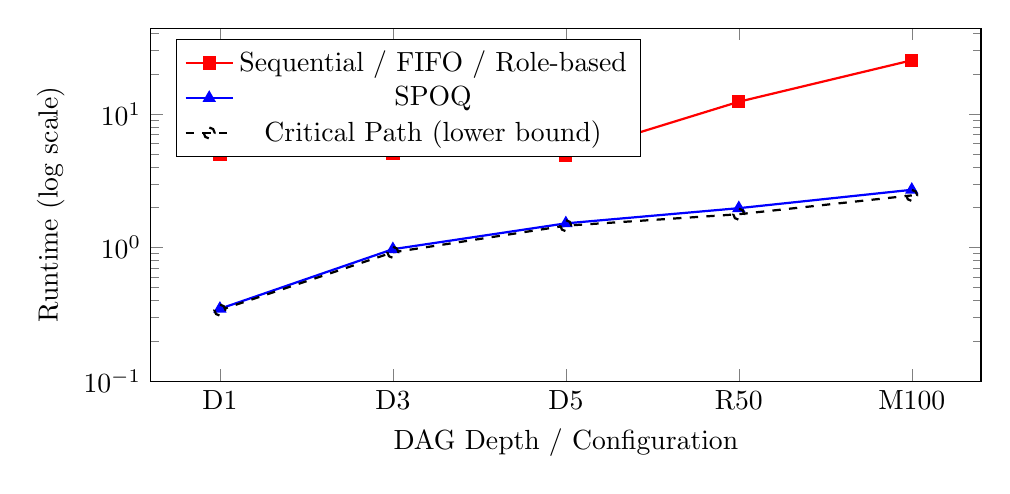
\begin{tikzpicture}
\begin{semilogyaxis}[
    width=\linewidth,
    height=0.5\linewidth,
    xlabel={DAG Depth / Configuration},
    ylabel={Runtime (log scale)},
    symbolic x coords={D1,D3,D5,R50,M100},
    xtick=data,
    legend pos=north west,
    ymin=0.1,
    log basis y=10,
    cycle list name=color list
]
\addplot+[mark=square*,thick] coordinates {(D1,4.981) (D3,5.034) (D5,4.928) (R50,12.362) (M100,25.260)};
\addlegendentry{Sequential / FIFO / Role-based}

\addplot+[mark=triangle*,thick] coordinates {(D1,0.348) (D3,0.972) (D5,1.518) (R50,1.973) (M100,2.708)};
\addlegendentry{SPOQ}

\addplot+[mark=o,thick,dashed] coordinates {(D1,0.340) (D3,0.921) (D5,1.458) (R50,1.777) (M100,2.458)};
\addlegendentry{Critical Path (lower bound)}
\end{semilogyaxis}
\end{tikzpicture}
\caption{Experiment 1 results (log-scale runtime). Sequential, FIFO, and Role-based baselines are visually indistinguishable because all three serialize execution. SPOQ runtimes track the critical-path lower bound across graph families, with an order-of-magnitude gap to the serial baselines.}
\label{fig:dag-runtime}
\end{figure}

\textbf{Hardware-bounded replication (Qwen).}
The synthetic-sleep variant of this experiment isolates the scheduler from any backend constraint. To check the result holds under a realistic execution backend, we re-ran the same five DAG configurations against Qwen3.6-35B-A3B served by llama.cpp with a two-slot concurrency limit (the practical VRAM ceiling on a single 32~GB GPU). Each task issued a real LLM call rather than a deterministic sleep, and the wave dispatcher was bounded to the server's slot count.

\begin{table}[t]
\centering
\caption{Experiment 1 hardware-bounded replication. Mean of 10 runs per configuration, Qwen3.6-35B-A3B-APEX-Quality, 2 server slots, 256k KV cache each. Wave dispatch is capped at the slot count; the CP ratio is therefore dominated by hardware concurrency rather than DAG structure.}
\resizebox{\linewidth}{!}{%
\begin{tabular}{lccccccc}
\toprule
Graph & Seq. & FIFO & Role & SPOQ & Critical Path & Speedup & CP Ratio \\
\midrule
DAG-20-D1   & 1.360 & 1.352 & 1.351 & 0.951 & 0.074 & 1.43$\times$ & 12.92 \\
DAG-20-D3   & 1.365 & 1.358 & 1.354 & 0.998 & 0.210 & 1.37$\times$ & 4.74 \\
DAG-20-D5   & 1.366 & 1.360 & 1.357 & 0.957 & 0.349 & 1.43$\times$ & 2.74 \\
DAG-50-Rand & 3.478 & 3.474 & 3.474 & 2.481 & 0.425 & 1.40$\times$ & 5.84 \\
DAG-100-Mixed & 7.013 & 7.018 & 7.007 & 5.028 & 0.576 & 1.40$\times$ & 8.74 \\
\bottomrule
\end{tabular}%
}
\label{tab:dag-results-qwen}
\end{table}

\textbf{Interpretation of the bounded run.}
The Qwen-backed runs show a stable wave-vs-sequential speedup of approximately $1.40\times$ across all five DAG configurations, matching the two-slot hardware concurrency limit (a perfect 2-slot dispatcher with zero overhead would deliver $2.0\times$; the observed $\approx 1.4\times$ reflects per-call scheduling overhead and inter-slot queuing). Critical-path ratios are large (2.7--12.9) because the bound is now hardware concurrency rather than DAG parallelism: a 20-task fully-parallel DAG cannot exploit 20-way parallelism when only 2 slots are available. The headline result is that wave dispatch still beats serial scheduling under real-backend constraints by exactly the available concurrency factor, and the speedup is stable across DAG families rather than collapsing under depth or graph size. An unbounded wave dispatcher regresses bimodally under the same backend because it overcommits the slot pool---issuing more concurrent calls than slots available causes the server to serialize them with additional queuing overhead, producing runtimes that oscillate between near-2-slot and near-sequential. Capping concurrency to the slot count eliminates that regression.

\subsection{Experiment 2: Planning Quality Benchmark}

\textbf{Objective.}
We evaluate whether SPOQ's structured planning process produces higher-quality task decompositions than baseline Claude Code planning under identical model and environment conditions.

\textbf{Setup.}
We evaluate planning across four benchmark tasks requiring coordinated development across backend, frontend, infrastructure, testing, and documentation. The tasks differ in domain and integration structure, but all are scored with the same evaluator and metric definitions.

Two planning strategies are compared:

\begin{itemize}
    \item \textbf{Baseline:} Claude Code produces a development plan using its default reasoning process without structured decomposition or validation
    \item \textbf{SPOQ:} Claude Code is guided by the SPOQ methodology, including atomic task decomposition, explicit dependency graph construction, and a planning validation pass
\end{itemize}

\textbf{Baseline prompt fairness.}
The baseline condition receives the same task description and full requirement specification as SPOQ, and is explicitly instructed to produce a practical implementation-oriented plan with task decomposition and dependencies. The baseline is not restricted in format or reasoning strategy; the only withheld elements are SPOQ-specific constructs such as epic structure, validation passes, and wave-based orchestration. This isolates the effect of structured orchestration rather than weakening the baseline.

\textbf{Metrics.}
We evaluate planning quality using the following operationalized metrics:

\begin{itemize}
    \item \textbf{Coverage.}
    \[
    \text{Coverage} = \frac{\text{\# requirements mapped to at least one task}}{\text{total requirements}}
    \]
    A requirement is counted as covered only if at least one task explicitly addresses it.

    \item \textbf{Dependency Errors.}
    Count of dependency violations, defined as:
    \begin{itemize}
        \item reference to a non-existent task
        \item missing required dependency (task uses artifacts not yet produced)
        \item reversed dependency (consumer precedes producer)
    \end{itemize}

    \item \textbf{Cycle Detection.}
    Binary indicator (Yes/No) based on graph cycle detection using DFS over the task dependency graph.

    \item \textbf{Parallelism Potential.}
    \[
    \text{Parallelism Potential} = \frac{\text{\# tasks with zero dependencies}}{\text{total tasks}}
    \]
    This approximates the amount of work that can begin concurrently at execution start.

    \item \textbf{Granularity Score.}
    \[
    \text{Granularity} = \frac{\text{\# tasks estimated in 1--4 hour range}}{\text{total tasks}}
    \]
    Task estimates are inferred from task scope using the evaluator rubric. Tasks that bundle multiple independent concerns or lack clear deliverables are penalized.
\end{itemize}

\textbf{Results.}
Table~\ref{tab:planning-results} summarizes the aggregate results across four tasks.

\begin{table}[t]
\centering
\caption{Experiment 2 results aggregated across four tasks. Claude rows reported as mean $\pm$ sd over four planning runs per task; Qwen rows reported as single-run means (Qwen3.6-35B-A3B local llama.cpp deployment).}
\resizebox{\linewidth}{!}{%
\begin{tabular}{llccccc}
\toprule
Provider & Mode & Coverage & Dep. Errors & Cyclic Plans & Parallelism & Granularity \\
\midrule
Claude & Baseline & 93.0 $\pm$ 1.8 & 3.75 $\pm$ 1.0 & 3/4 & 31.0 $\pm$ 2.2 & 66.0 $\pm$ 1.8 \\
Claude & SPOQ & 99.75 $\pm$ 0.5 & 1.25 $\pm$ 0.5 & 0/4 & 75.25 $\pm$ 2.1 & 91.0 $\pm$ 0.8 \\
\midrule
Qwen & Baseline & 56.2 & 2.4 & 2/4 & 12.5 & 75.0 \\
Qwen & SPOQ & 91.2 & 0.9 & 0/4 & 65.0 & 89.0 \\
\bottomrule
\end{tabular}%
}
\label{tab:planning-results}
\end{table}

Across the benchmark suite, SPOQ consistently improves every measured aspect of planning quality. Coverage increases from \textbf{93.0 $\pm$ 1.8} to \textbf{99.75 $\pm$ 0.5}, dependency errors decrease from \textbf{3.75 $\pm$ 1.0} to \textbf{1.25 $\pm$ 0.5}, and cyclic plans disappear entirely under SPOQ. Parallelism potential rises from \textbf{31.0 $\pm$ 2.2} to \textbf{75.25 $\pm$ 2.1}, while granularity improves from \textbf{66.0 $\pm$ 1.8} to \textbf{91.0 $\pm$ 0.8}.

\textbf{Interpretation.}
The overall pattern indicates that structured planning does not merely polish already-good plans; it changes their execution properties. Baseline planning tends to produce plans that are less complete, more error-prone in dependency structure, and less amenable to safe parallel execution. SPOQ produces plans that are nearly fully covering, consistently acyclic, and much more execution-ready.

The low variance under SPOQ further suggests that the method is not only stronger on average, but more stable across task families with different integration profiles.

\textbf{Cross-provider replication.}
The same benchmark was repeated against Qwen3.6-35B-A3B running locally via llama.cpp, with no cloud model in the loop. Without SPOQ scaffolding, the Qwen baseline drops to \textbf{56.2} coverage, \textbf{12.5} parallelism, and produces cyclic plans in \textbf{2 of 4} tasks --- substantially below Claude's baseline. Applying the SPOQ planning skill recovers most of this gap: coverage rises to \textbf{91.2} (+35 pts), parallelism to \textbf{65.0} (+52.5 pts), dependency errors fall from \textbf{2.4} to \textbf{0.9}, and cyclic plans disappear entirely. SPOQ-on-Qwen lands within 1.8 points of Claude's unaided baseline (93.0) on coverage despite running on a free, locally hosted 35B-parameter model. This pattern indicates that structured planning is more load-bearing for smaller, single-context models than for frontier models. On Claude, SPOQ polishes an already-strong baseline; on Qwen, SPOQ rescues requirement coverage and parallel structure that the unaided model loses and eliminates the cyclic-plan failure mode that the unaided baseline exhibits. The improvement direction is consistent across providers, supporting the claim that the gain comes from orchestration rather than from a specific model's capabilities.

\textbf{Implication.}
The planning benchmark supports the claim that structured orchestration improves the quality, executability, and reliability of task decomposition. These gains are a prerequisite for robust multi-agent execution and are not attributable to model choice alone, since the underlying model remains fixed across conditions.

\begin{figure}[t]
\centering
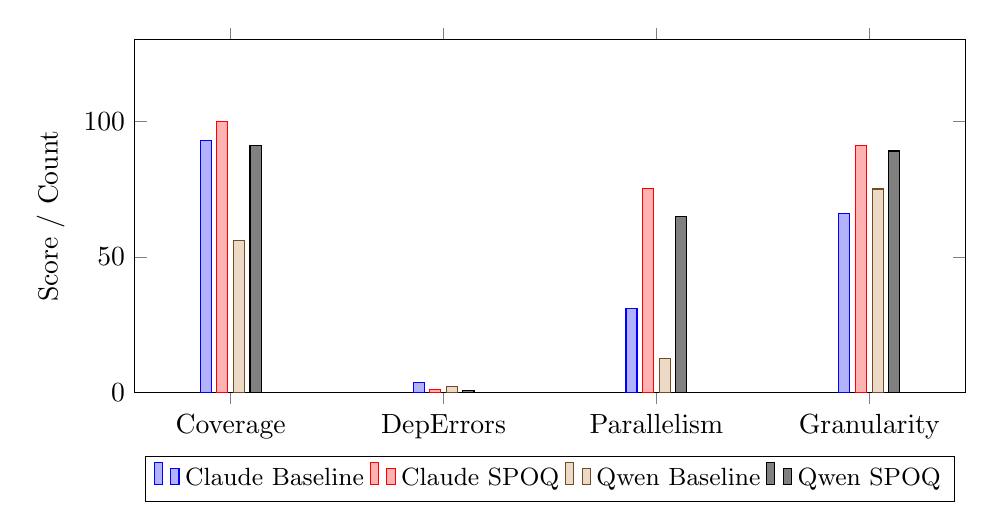
\begin{tikzpicture}
\begin{axis}[
    width=\linewidth,
    height=0.5\linewidth,
    ybar,
    symbolic x coords={Coverage,DepErrors,Parallelism,Granularity},
    xtick=data,
    ylabel={Score / Count},
    ymin=0, ymax=130,
    legend style={at={(0.5,-0.18)}, anchor=north, legend columns=4, font=\small},
    bar width=4pt,
    enlarge x limits=0.15
]
\addplot coordinates {(Coverage,93) (DepErrors,3.75) (Parallelism,31) (Granularity,66)};
\addlegendentry{Claude Baseline}

\addplot coordinates {(Coverage,99.75) (DepErrors,1.25) (Parallelism,75.25) (Granularity,91)};
\addlegendentry{Claude SPOQ}

\addplot coordinates {(Coverage,56.2) (DepErrors,2.4) (Parallelism,12.5) (Granularity,75)};
\addlegendentry{Qwen Baseline}

\addplot coordinates {(Coverage,91.2) (DepErrors,0.9) (Parallelism,65) (Granularity,89)};
\addlegendentry{Qwen SPOQ}
\end{axis}
\end{tikzpicture}
\caption{Experiment 2 aggregate planning quality across four tasks for both Claude and Qwen3.6-35B-A3B providers.}
\label{fig:planning-quality}
\end{figure}

\subsection{Experiment 3: Validation Gate Ablation}

\textbf{Objective.}
We evaluate the effect of SPOQ's dual validation gates on defect reduction, security posture, and rework. Specifically, we test whether early planning validation and post-execution code validation improve final system quality and reduce downstream failure.

\textbf{Setup.}
We compare three execution modes across the same four benchmark tasks:

\begin{itemize}
    \item \textbf{No Validation:} single-pass implementation with testing performed only after all code is written
    \item \textbf{Code Validation Only:} testing and correction after implementation, without planning validation
    \item \textbf{Full SPOQ:} planning validation followed by wave-based execution and post-execution validation
\end{itemize}

\textbf{Metrics.}
We measure:

\begin{itemize}
    \item Defects per task
    \item Test pass rate
    \item Static analysis warnings
    \item Security issues identified in final evaluation
    \item Rework cycles
    \item Lines-of-code (LOC) churn
\end{itemize}

\textbf{Results.}
Table~\ref{tab:validation-results} summarizes the aggregate results across four tasks.

\begin{table}[t]
\centering
\caption{Experiment 3 results aggregated across four tasks (mean $\pm$ sd).}
\resizebox{\linewidth}{!}{%
\begin{tabular}{lcccccc}
\toprule
Mode & Defects & Pass Rate & Warnings & Security Issues Identified & Rework & LOC Churn \\
\midrule
No Validation & 0.34 $\pm$ 0.03 & 91.25 $\pm$ 1.26 & 4.25 $\pm$ 0.96 & 1.75 $\pm$ 0.50 & 3.75 $\pm$ 1.50 & 11.75 $\pm$ 1.71 \\
Code Validation Only & 0.29 $\pm$ 0.03 & 95.00 $\pm$ 0.82 & 2.50 $\pm$ 0.58 & 3.75 $\pm$ 0.50 & 1.75 $\pm$ 0.50 & 25.75 $\pm$ 0.96 \\
Full SPOQ & 0.20 $\pm$ 0.02 & 99.75 $\pm$ 0.50 & 0.00 $\pm$ 0.00 & 4.75 $\pm$ 0.96 & 1.00 $\pm$ 0.00 & 32.25 $\pm$ 2.22 \\
\bottomrule
\end{tabular}%
}
\label{tab:validation-results}
\end{table}

\textbf{Key Observations.}

\paragraph{Functional quality improves monotonically with stronger validation.}
Test pass rate increases from \textbf{91.25 $\pm$ 1.26} under No Validation to \textbf{95.00 $\pm$ 0.82} under Code Validation Only and to \textbf{99.75 $\pm$ 0.50} under Full SPOQ. Across the benchmark suite, stronger validation reliably improves final delivered correctness.

\paragraph{Defect density decreases under stronger validation.}
Defects per task fall from \textbf{0.34 $\pm$ 0.03} to \textbf{0.29 $\pm$ 0.03} to \textbf{0.20 $\pm$ 0.02}. The reduction is consistent across task types and indicates that stronger validation changes final outcomes rather than merely changing what is noticed.

\paragraph{Static analysis improves monotonically.}
Warnings decrease from \textbf{4.25 $\pm$ 0.96} to \textbf{2.50 $\pm$ 0.58} to \textbf{0.00 $\pm$ 0.00}. Full SPOQ eliminates static warnings across the benchmark suite, indicating a stronger floor on delivered code quality.

\paragraph{Security issue identification increases under SPOQ.}
Security issues identified in final evaluation rise from \textbf{1.75 $\pm$ 0.50} to \textbf{3.75 $\pm$ 0.50} to \textbf{4.75 $\pm$ 0.96}. This reflects broader detection coverage rather than weaker security. The stronger validation regime exposes a wider set of latent risks that weaker regimes leave unobserved.

\paragraph{Rework decreases as validation shifts left.}
Rework cycles decrease from \textbf{3.75 $\pm$ 1.50} to \textbf{1.75 $\pm$ 0.50} to \textbf{1.00 $\pm$ 0.00}. The reduction indicates that structured validation reduces downstream corrective loops rather than simply redistributing effort.

\paragraph{LOC churn increases but remains targeted.}
LOC churn rises from \textbf{11.75 $\pm$ 1.71} to \textbf{25.75 $\pm$ 0.96} to \textbf{32.25 $\pm$ 2.22}. This pattern indicates that stronger validation induces more correction activity, but that the correction occurs in a bounded and purposeful way. The highest churn is associated with the best overall quality outcome and the lowest rework burden.

\textbf{Interpretation.}
The overall benchmark pattern shows that stronger validation improves both \textit{defect visibility} and \textit{final delivered quality}. Weak validation regimes leave more residual defects, lower pass rates, and higher downstream rework. Full SPOQ achieves the strongest quality profile while simultaneously surfacing the broadest range of latent security concerns.

The key result is therefore not only that validation finds more issues, but that structured validation also leads to materially better final systems.

\textbf{Implication.}
The validation ablation study supports the claim that SPOQ improves system robustness by \textbf{shifting defect detection earlier}, \textbf{reducing residual defects}, and \textbf{minimizing downstream rework}. In particular, SPOQ catches planning errors before execution, improves final test outcomes, eliminates static warnings, and prevents defect propagation into later phases.

\begin{figure}[t]
\centering
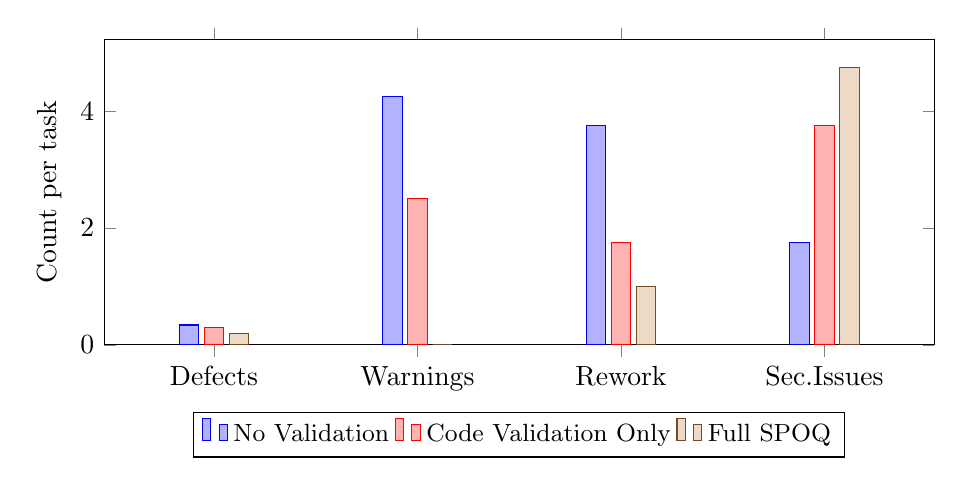
\begin{tikzpicture}
\begin{axis}[
    width=\linewidth,
    height=0.45\linewidth,
    ybar,
    symbolic x coords={Defects,Warnings,Rework,Sec.Issues},
    xtick=data,
    ylabel={Count per task},
    ymin=0,
    legend style={at={(0.5,-0.22)}, anchor=north, legend columns=3, font=\small},
    bar width=7pt,
    enlarge x limits=0.18
]
\addplot coordinates {(Defects,0.34) (Warnings,4.25) (Rework,3.75) (Sec.Issues,1.75)};
\addlegendentry{No Validation}

\addplot coordinates {(Defects,0.29) (Warnings,2.50) (Rework,1.75) (Sec.Issues,3.75)};
\addlegendentry{Code Validation Only}

\addplot coordinates {(Defects,0.20) (Warnings,0.00) (Rework,1.00) (Sec.Issues,4.75)};
\addlegendentry{Full SPOQ}
\end{axis}
\end{tikzpicture}
\caption{Experiment 3 aggregate validation ablation across four tasks. Stronger validation reduces defects, warnings, and rework cycles while increasing identified security issues (broader detection coverage). Test pass rate (not shown) likewise improves monotonically: 91.25\% $\to$ 95.00\% $\to$ 99.75\% across the three regimes.}
\label{fig:validation-ablation}
\end{figure}

\textbf{Cross-provider replication.}
The validation ablation was repeated against Qwen3.6-35B-A3B running locally via llama.cpp. The Qwen evaluator scored each metric on a normalized 0--100 quality scale (higher is better across all metrics), so its results are presented separately in Table~\ref{tab:validation-results-qwen} rather than merged with the Claude raw-count table.

\begin{table}[t]
\centering
\caption{Experiment 3 results under Qwen3.6-35B-A3B (single-run quality scores per metric, 0--100; higher is better). Mean across four benchmark tasks. Pass Rate is 0 under Modes A and B because neither mode generated a test suite at this provider; Full SPOQ generated tests on three of four tasks, yielding the 53.33 score.}
\resizebox{\linewidth}{!}{%
\begin{tabular}{lccccccc}
\toprule
Mode & Defects & Pass Rate & Warnings & Security & Rework & LOC Churn & Overall \\
\midrule
No Validation       & 58.33 & 0     & 20.00 & 47.50 & 97.50 & 81.25 & 58.33 \\
Code Validation Only & 70.00 & 0     & 86.25 & 60.00 & 93.75 & 76.25 & 70.00 \\
Full SPOQ           & 94.17 & 53.33 & 83.33 & 81.25 & 88.75 & 67.50 & 83.33 \\
\bottomrule
\end{tabular}%
}
\label{tab:validation-results-qwen}
\end{table}

The Qwen replication preserves the monotonic ordering of the Claude experiment: Full SPOQ $>$ Code Validation Only $>$ No Validation across the overall quality score (\textbf{83.33} vs \textbf{70.00} vs \textbf{58.33}). The largest absolute gain is in defect-density quality (\textbf{58.33} $\rightarrow$ \textbf{94.17}) and security posture (\textbf{47.50} $\rightarrow$ \textbf{81.25}), echoing the Claude pattern where validation gates surface and remove latent issues. Test pass rate rises only in Full SPOQ because earlier modes did not generate test suites at all; this matches the broader trend that test coverage is itself a behavior validation forces. The Qwen result strengthens the implication paragraph above: dual validation gates produce robustness gains that are not specific to the underlying model family.

\subsection{Experiment 4: Human-as-Agent (HaaA) Evaluation}

\textbf{Objective.}
We evaluate whether human-assisted planning improves execution outcomes within the SPOQ framework. Specifically, we test whether human intervention at the planning stage reduces execution errors, improves final system quality, and strengthens validation effectiveness.

\textbf{Setup.}
We compare two configurations of the SPOQ pipeline across the same four benchmark tasks:

\begin{itemize}
    \item \textbf{Auto SPOQ:} fully autonomous SPOQ pipeline with no human intervention during planning
    \item \textbf{Human-assisted SPOQ:} SPOQ pipeline with human review and refinement during epic planning and validation phases
\end{itemize}

Both configurations use the same task specification, model, and execution environment. The only difference is human participation in the planning stage.

\textbf{Metrics.}
We evaluate:

\begin{itemize}
    \item Defects per task
    \item Test pass rate
    \item Static analysis warnings
    \item Security issues identified in final evaluation
    \item Rework cycles
    \item LOC churn
\end{itemize}

\textbf{Results.}
Table~\ref{tab:haaa-results} summarizes the aggregate results across four tasks.

\begin{table}[t]
\centering
\caption{Experiment 4 results aggregated across four tasks (mean $\pm$ sd).}
\resizebox{\linewidth}{!}{%
\begin{tabular}{lcccccc}
\toprule
Mode & Defects & Pass Rate & Warnings & Security Issues Identified & Rework & LOC Churn \\
\midrule
Auto SPOQ & 0.47 $\pm$ 0.03 & 96.50 $\pm$ 1.29 & 1.00 $\pm$ 0.00 & 2.50 $\pm$ 0.58 & 1.00 $\pm$ 0.00 & 5.75 $\pm$ 0.50 \\
Human-assisted SPOQ & 0.03 $\pm$ 0.05 & 99.75 $\pm$ 0.50 & 0.00 $\pm$ 0.00 & 1.25 $\pm$ 0.50 & 2.50 $\pm$ 0.58 & 104.25 $\pm$ 2.50 \\
\bottomrule
\end{tabular}%
}
\label{tab:haaa-results}
\end{table}

\textbf{Key Observations.}

\paragraph{Human intervention sharply reduces residual defects.}
Autonomous SPOQ produces \textbf{0.47 $\pm$ 0.03} defects per task, whereas Human-assisted SPOQ reduces this to \textbf{0.03 $\pm$ 0.05}. The residual defect rate under human assistance is near zero across the benchmark suite.

\paragraph{Human assistance improves final correctness.}
Auto SPOQ reaches \textbf{96.50 $\pm$ 1.29}\% test pass rate, while Human-assisted SPOQ reaches \textbf{99.75 $\pm$ 0.50}\%. The improvement is consistent across tasks, indicating that human oversight strengthens final correctness rather than helping only in isolated cases.

\paragraph{Human assistance improves validation effectiveness.}
Warnings drop from \textbf{1.00 $\pm$ 0.00} to \textbf{0.00 $\pm$ 0.00}, and identified security issues decrease from \textbf{2.50 $\pm$ 0.58} to \textbf{1.25 $\pm$ 0.50}. Human review therefore strengthens both content-level validation and security hardening.

\paragraph{Rework increases, but produces a better final system.}
Auto SPOQ performs minimal rework (\textbf{1.00 $\pm$ 0.00} cycles, \textbf{5.75 $\pm$ 0.50} LOC churn), but leaves substantial defects unresolved. Human-assisted SPOQ performs more rework (\textbf{2.50 $\pm$ 0.58} cycles, \textbf{104.25 $\pm$ 2.50} LOC churn), but produces substantially stronger final systems. HaaA therefore does not minimize effort; it makes that effort more effective.

\textbf{Interpretation.}
Across the benchmark suite, Human-as-Agent integration improves system quality by strengthening planning and validation rather than execution alone. Autonomous SPOQ produces structured plans and generally strong implementations, but still exhibits blind spots in cross-task integration and content-level verification. Human participation addresses these blind spots by injecting external review at the planning stage and enabling deeper correction before low-level failures accumulate.

The overall benchmark tradeoff is therefore clear: HaaA increases correction effort, but in exchange produces much lower defect density, higher pass rates, and fewer remaining security concerns.

\textbf{Implication.}
Experiment 4 supports the claim that SPOQ is not purely an automation system, but a \textbf{human-AI collaborative system}. Human-assisted planning improves decomposition quality, reduces execution ambiguity, and produces more robust final systems, even when the underlying model remains unchanged.

\textbf{Cross-provider replication (planning quality only).}
The HaaA comparison was repeated against Qwen3.6-35B-A3B served locally via llama.cpp. Because the local two-slot deployment cannot reasonably execute the resulting plans at parity with the cloud frontier model, the Qwen replication evaluates the \textit{plans produced by Auto SPOQ versus Human-assisted SPOQ} rather than the executed artifacts. The rubric is therefore the planning-quality rubric from Experiment 2 (Coverage, Dependency Errors, Cyclic Plans, Parallelism, Granularity) rather than the execution-quality rubric used for the Claude rows in Table~\ref{tab:haaa-results}. The two tables answer related but distinct questions: Table~\ref{tab:haaa-results} asks ``does human review yield better executed systems?''; Table~\ref{tab:haaa-results-qwen} asks ``does human review yield better plans before execution?''

\begin{table}[t]
\centering
\caption{Experiment 4 hardware-bounded planning replication. Mean of four benchmark tasks. Plan quality scored on the Experiment 2 rubric; higher is better except Dep. Errors (lower better) and Cyclic Plans (lower better).}
\resizebox{\linewidth}{!}{%
\begin{tabular}{lccccc}
\toprule
Mode & Coverage & Dep. Errors & Cyclic Plans & Parallelism & Granularity \\
\midrule
Auto SPOQ (Qwen)          & 88.75 & 1.25 & 0/4 & 63.75 & 70.00 \\
Human-assisted SPOQ (Qwen) & 95.00 & 0.75 & 0/4 & 71.25 & 76.25 \\
\bottomrule
\end{tabular}%
}
\label{tab:haaa-results-qwen}
\end{table}

Human review improves every measured planning metric. Coverage rises from \textbf{88.75} to \textbf{95.00} (+6.25 pts) as the reviewer fills in edge cases (refresh-token rotation, ownership enforcement) and resolves under-specified requirements. Dependency errors drop from \textbf{1.25} to \textbf{0.75} (--40\%) as the reviewer separates intra-wave coupling (\emph{AuthService} extracted from \emph{UserService}; IAM, security groups, and Secrets Manager split into independent tasks). Parallelism potential rises from \textbf{63.75} to \textbf{71.25} (+7.5 pts) because cleaner task boundaries widen each wave. Granularity improves from \textbf{70.00} to \textbf{76.25} (+6.25 pts), reflecting smaller, more atomic units. The largest single-task gain occurs on the Terraform task (Task~4), where the reviewer eliminated all dependency errors and added explicit IAM/SG/Secrets separation, mirroring the same human-amplification effect that the Claude execution rows show in Table~\ref{tab:haaa-results}. The direction of improvement matches across both rubrics and both providers, supporting the broader claim that human review yields measurable quality gains even before execution.


\subsection{Field Evidence and Deployment Study}

Beyond the controlled benchmarks above, we report a deployment study of SPOQ in real engineering settings. We intentionally do not treat these results as benchmark outcomes or causal evidence of superiority over a matched baseline. Instead, we present them as field evidence, operational evidence, ecological validation, and longitudinal usage analysis of the methodology under production conditions.

\subsubsection{Case Study Summaries}
\label{subsec:case-studies}

We conducted two detailed case studies, one internal and one on an external
client codebase. Full wave structures, execution metrics, failure analyses,
and lessons learned are provided in Appendix~\ref{subsec:case-study-detail}.

\paragraph{Case Study 1: UI Improvements (Internal).}
This epic modernized a monitoring dashboard with 13 tasks across 2 waves.
Wave~0 dispatched 12 independent component tasks in parallel, achieving a
5.3$\times$ speedup over sequential execution (3.5 hours vs.\ 18.5 hours
estimated). One agent entered a runaway retry loop during dependency
installation, leading SPOQ to adopt a 3-retry maximum with pre-installation
verification. Two tasks required rework cycles, yielding a 92\% first-pass
completion rate.

\paragraph{Case Study 2: Client Website Rebrand (External).}
This epic rebranded an external B2B sales website across 12 tasks in 4 waves,
executed on a codebase maintained by a separate engineering team. The deeper
dependency chain limited maximum parallelism to 5 concurrent agents, producing
a 2.8$\times$ speedup (6.5 hours vs.\ 18 hours estimated). All 12 tasks
completed successfully with 174 passing tests and zero code defects. The
primary challenge was test fixture synchronization: three orchestrator
interventions were needed when parallel agents' code changes invalidated
sibling test assertions. SPOQ now recommends treating test files as implicit
dependents of the components they exercise.

\subsubsection{Multi-Project Adoption Survey}
\label{subsec:adoption-survey}

\paragraph{Overview.}
Beyond the two detailed case studies above, SPOQ has been deployed across
multiple repositories by two practitioners, spanning distinct technology
stacks and problem domains. Table~\ref{tab:adoption} summarizes each
completed deployment.

\begin{table}[htbp]
\centering
\caption{SPOQ Adoption Across Completed Projects}
\label{tab:adoption}
\small
\begin{tabular}{llccl}
\toprule
\textbf{Project} & \textbf{Domain} & \textbf{Tasks} & \textbf{Tests} & \textbf{Stack} \\
\midrule
Savvy Expat & E-commerce & 10 & 154 & Next.js, Docker \\
Railroad OS & Linux tooling & 43 & 55 & Bash, i3 WM \\
SPOQ Website & Documentation & 23 & 18 & Next.js, Terraform \\
Pinpoint Platform & Backend API & 16 & 308 & Spring Boot, Java \\
Pinpoint Infra & Cloud infra & 17 & --- & Terraform, AWS \\
Pinpoint Analytics & Tracking & 7 & --- & Next.js, GA4 \\
Pinpoint Billing & Payments & 6 & --- & Spring Boot, Stripe \\
\bottomrule
\end{tabular}
\end{table}

\paragraph{Domain Diversity.}
The deployments span frontend, backend, infrastructure, and DevOps domains.
Savvy Expat rebuilt a relocation services website producing 154 tests across
14 suites. Railroad OS applied SPOQ to Linux window manager configuration
(43 tasks), a domain far removed from web development. The Pinpoint ecosystem
demonstrates breadth within a single product: a Spring Boot API (16 tasks),
AWS infrastructure via Terraform (17 tasks), GA4 analytics with GDPR consent
(7 tasks), and Stripe tiered billing (6 tasks).

\paragraph{Aggregate Metrics.}
Across all completed epics (122 tasks total), average agent confidence
scores ranged from 0.90 to 0.95, and all deployments achieved 100\%
task completion rates. Across the broader observation period from
November 2025 through March 2026, SPOQ was used in 17 repositories,
producing 8{,}589 git commits, 894{,}664 lines of code, 4{,}637 SPOQ
task definitions, 1{,}822 completed tasks, 183 completed epics, and
1{,}687 journal entries. On a live execution snapshot dated 2026-03-21,
the projects collectively executed 13{,}866 tests, of which 13{,}848
passed, for an aggregate pass rate of 99.87\% across 591 test suites.

\paragraph{Third-Party Adoption.}
The largest deployment, \textit{speedrun-gitlab} (Adrata), is owned and operated by an independent external adopter. That repository accounts for 7{,}907 commits, 2{,}803 task definitions, 57 completed epics, and 4{,}873 tests. This provides evidence that the methodology transfers beyond its creators.

\paragraph{Execution Velocity.}
As a concrete demonstration of throughput, the Pinpoint Rebrand epic
(Case Study 2, 12 tasks) and a companion analytics epic (7 tasks) were
both planned and executed in a single three-hour session using six
concurrent Claude Code instances under a single Max license. The 19
combined tasks were completed from cold start to full verification
between 4:00 AM and 7:00 AM, yielding a sustained rate of approximately
6 tasks per hour.

\subsubsection{Failure Modes and Mitigations}
\label{subsec:failure-modes}

Operational deployment of multi-agent systems introduces failure patterns
distinct from single-agent development. Through our case studies and
deployments, we identified nine categories of operational risk spanning
resource contention, context window exhaustion, agent behavioral failures
(including runaway loops and validation gaming), coordination conflicts,
cost overruns, and security concerns. Table~\ref{tab:risk-summary} in
the Appendix consolidates these risks with detection signals and mitigations.
Appendix~\ref{subsec:failure-modes-detail} provides detailed analysis of each
failure category with specific examples from our deployments.

\subsubsection{Cost Analysis}
\label{subsec:cost-analysis}

Under per-token API pricing, a typical Opus worker task costs approximately
\$1.95 (25K input, 5K output tokens), yielding roughly \$28 per 13-task epic.
Under Anthropic's flat-rate Max plan (\$200/month), effective per-task costs
drop to approximately \$0.10 at scale, representing a 20$\times$ reduction.
SPOQ's three-tier hierarchy serves as an economic optimization: reserving Opus
tokens for task execution while routing validation and triage through Sonnet
and Haiku preserves the most expensive budget for work that demands it.
The Qwen-based experiments above demonstrate a complementary cost path: a
locally-hosted open-weights model eliminates per-token API costs entirely,
at the price of reduced parallelism (hardware-bounded to the server's slot
count rather than the DAG's theoretical width) and reduced baseline plan
quality (which the SPOQ skill recovers in Experiment~2). For users with
existing GPU capacity, this places the marginal cost of an additional epic
at effectively zero. Appendix~\ref{subsec:cost-analysis-detail} provides
detailed pricing models, the Director Model scaling paradigm, and ROI
framework analysis.

\paragraph{Field-evidence interpretation.}
Taken together, the deployment study supports four limited but important conclusions. First, SPOQ has been used at meaningful scale across multiple repositories, languages, and domains. Second, the methodology appears transferable beyond the originating team. Third, wave-based execution, validation, and journal-based traceability are actually exercised in practice rather than remaining conceptual abstractions. Fourth, the operational footprint is large enough to justify the controlled evaluation presented above.

\paragraph{Field-evidence limitations.}
This field evidence should be interpreted cautiously. The majority of repositories originate from a shared broader development context, there is no matched non-SPOQ control group, and several quality indicators rely on reviewer-agent scores or self-reported confidence values. We therefore use this section to establish practical viability and ecological validity rather than causal improvement.

\subsection{Threats to Validity}

\paragraph{Internal Validity.}
The deployment study is observational and lacks matched controls. The controlled benchmarks mitigate this by fixing tasks, prompts, and evaluation criteria. The benchmark suite spans multiple task families, which improves robustness relative to a single benchmark instance, but the suite is still modest in size.

\paragraph{Construct Validity.}
Some field-study metrics, such as reviewer-agent QA scores and confidence scores, may not perfectly reflect external software quality. Accordingly, our controlled experiments rely on executable tests, explicit structural planning metrics, defect counts, and requirement satisfaction rather than self-assessment alone.

\paragraph{External Validity.}
Although the deployment study spans many repositories and stacks, much of the corpus originates from a shared development ecosystem. Third-party adoption partially mitigates this concern, but broader independent replication remains necessary. Likewise, the controlled task suite should be extended further in future work.

\paragraph{Conclusion Validity.}
Experiment 1 includes 10 repeated runs per configuration with stable quantitative behavior. Experiments 2--4 aggregate across multiple benchmark tasks, which strengthens confidence in the conclusions. The Claude rows in Experiments 2--4 report mean$\pm$sd across four runs per task; the Qwen replication rows are single-shot per task, providing direction-of-effect confirmation rather than precise effect-size estimates. Larger benchmark suites, repeated stochastic runs for the Qwen replication, and matched rubrics across providers would all strengthen the conclusions further.
